% 导言区
\documentclass{article}
\usepackage{ctex}  % 导入中文包
\usepackage{graphicx} % Required for inserting images
\usepackage[ruled]{algorithm2e}
\usepackage{amsmath}


\title{\centering{信道编码的最新进展}}
\author{张嘉伟,杨筠松}
\date{\today}

% 正文区
\begin{document}
\maketitle
\thispagestyle{empty} % 隐藏页眉和页脚
\newpage

\tableofcontents
\newpage

\section{引言}
1948年,在《通信的数学理论》中,香农首次提出了信道容量的极限 \cite{shannon1948},并指出在码率小于信道容量时,如果码长足够长,可以以任意小的错误率传递信息。这是第一次人们从理论上认识信道,并有了信道编码的最终目标——达到香农极限。经过多年的发展,信道编码领域涌现了许许多多的编码算法。其中比较常用的两种方法是:分组码与卷积码。由于信道编码不仅包含编码部分,还要考虑解码的复杂度。因此,构造好的编码算法一般有两类途径:一种是考虑增加码长,即增加分组码的码长或者卷积码的约束条件;二是采用极大似然概率译码。然而,这两者有着不可调和的矛盾:极大似然概率译码的译码复杂度将会随码长$n$的增加呈指数上升,也就是说,如果码长过长,会使得译码几乎不可能实现。但是在香农定理的信道编码定理的指引下,人们相信总能找到一个合适的编码方法达到香农极限。如图列出了这几十年中发展出的优秀的编码方法与成果。
\cite{yu2018channel}

\begin{figure}[h]
  \centering
  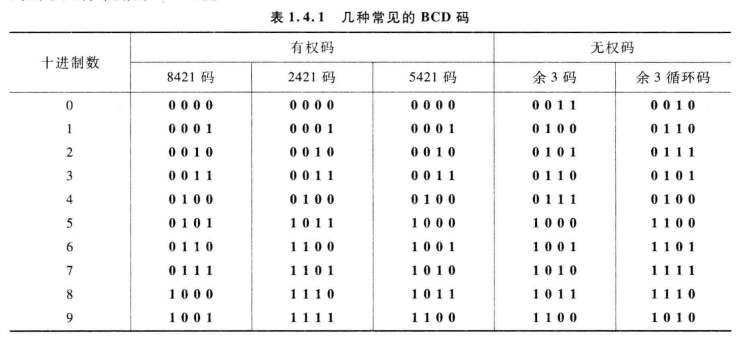
\includegraphics[width=\textwidth, keepaspectratio]{1-1.png}
  \caption{信道编码构造的重要发展历程}
\end{figure}

本文将简述信道编码的发展,并补充说明信道编码的基础知识,重点介绍现代信道编码的三个重大突破——LDPC码、Turbo码以及Polar码。

\section{信道编码基础知识概述}
\subsection{重复码、分组码与卷积码}
信道编码的本质是增加冗余以使得信道拥有检错和纠错能力,提高信道的稳定性。常见的有重复码、分组码与卷积码。
\subsubsection{重复码}
重复码就是简单地将每个信息比特重复,例如一个重复3次的重复码:$01\to000111$。接收端采用少数服从多数的方式进行解码,即当0个数超过一半时,认为发送端发送的是1,反之认为发送端发送的是0。即便重复码编解码方式简单,易于实现,但是传输效率低,一般不采用此方法。
\subsubsection{分组码}
分组码处理方法为:将信息序列每$k$个分为一组,每组按照设定的规则形成一个长度为$n$的码字,记为$(n,k)$分组码。
此时,可以将所用的码字看成一个码字空间,将使用的码字作为需用码字,不使用的码字作为禁用码字,码字空间可以由下图表示

\begin{figure}[h]
  \centering
  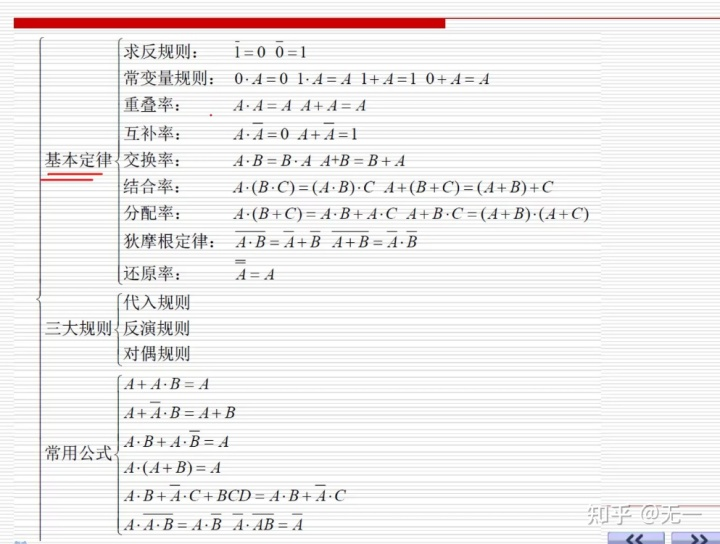
\includegraphics[width=0.8\textwidth, keepaspectratio]{2-1.png}
  \caption{禁用/可用码组与码字空间关系}
\end{figure}
其中禁用码组表示为$q^n-q^k$,可用码组为$q^k$以及码字空间为$q^n$,这样编码问题其实就转化为了选码问题,即在所有的码字中,选择一部分合适的码字作为许用码组。通常来说,许用码字之间的Hamming距离越大,即两个码字相同位置上不同码位的数目越多。纠错能力越强。

\subsubsection{卷积码}
分组码的局限性在于其忽略了各个码字之间的相关性,因此,卷积码应运而生。卷积码使用$(n, k, L)$表示,码率为$R$,其中$n$表示输出码字,$k$为输入的比特信息,$L$为约束长度也称为记忆深度,而$R$表示为$R = k/n$, 下图是一个最简单的$(2,1,2)$的卷积码编码器:

\begin{figure}[h]
  \centering
  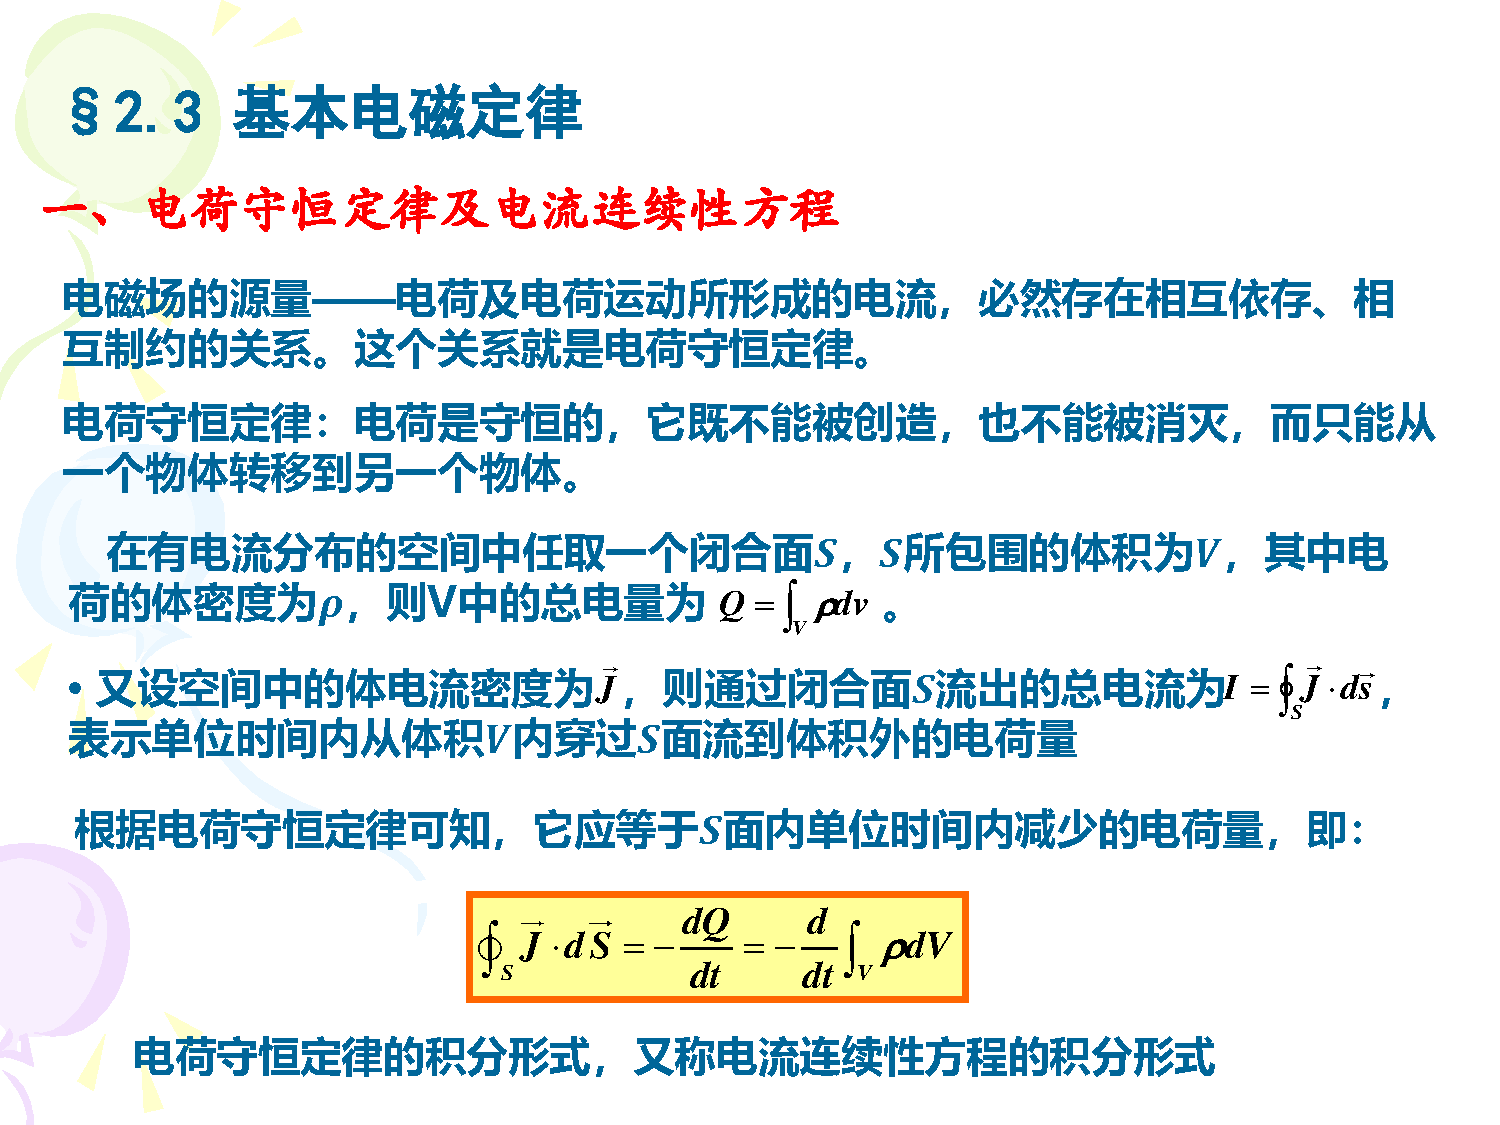
\includegraphics[width=0.8\textwidth, keepaspectratio]{2-2.png}
  \caption{(2,1,2)卷积码编码器}
\end{figure}

卷积码加入了记忆系统,将各个分组间的关系也纳入编码的考虑中。因此在对某一组编码时,还需要考虑这一组前若干组的输入,这大大提高了编码可靠性,但是相较于分组码,卷积码需要加入寄存器等记忆器件,使得实现的电路相对比较复杂。具体编码的伪代码如下所示:

\begin{algorithm}[H]
  \SetAlgoLined
  \SetKwFunction{Encode}{Encode}
  
  \KwData{Input message $m$, generator matrix $G$}
  \KwResult{Encoded message $c$}
  
  \BlankLine
  
  \caption{Convolutional Code Encoding}
  
  \BlankLine
  
  \SetKwProg{Function}{Function}{:}{}
  \Function{\Encode{$m$, $G$}}{
    $n \leftarrow$ number of bits per input symbol\;
    $k \leftarrow$ number of output bits per input symbol\;
    $N \leftarrow$ number of output symbols\;
    
    Initialize $c$ as an empty list\;
    
    \For{$i \leftarrow 0$ \KwTo $N-1$}{
      $u \leftarrow m[i]$ (extract input symbol)\;
      $x \leftarrow u \cdot G$ (matrix multiplication)\;
      
      \For{$j \leftarrow 0$ \KwTo $k-1$}{
        Append $x[j]$ to $c$\;
      }
    }
    
    \Return $c$\;
  }
  
\end{algorithm}

\subsection{最大似然译码}
最大似然译码是一种常用的信道编码译码方法。它基于接收到的信息$y$,计算所有可能的$P_{y|x_i}$,其中最大的值为其中最大的值对应的输入为$x^*$。通过比较不同可能性的概率,我们可以确定发送端发送的信息$x^*$ 。在实际应用中,通常我们只知道信道的统计特性(转移概率),而不知道信源的统计特性(输入概率)。因此,我们无法确定最佳译码规则,只能根据转移概率的某种约束条件制定译码规则。只有当信道输入等概时,最大似然译码规则才与最佳译码规则等价.

\subsection{交织器}
交织器的作用是将输入序列的顺序按照一定的规则进行打乱后再进行输出,即输出是输入的顺序重排。一般信道编码只能用于消除随机差错,对于突发差错没有纠错能力,使用交织器可以有效地抵御较长的突发噪声,将较长的突发噪声的影响平均分摊到每一个码字上,把突发噪声转变为随即噪声(如AWGN),此时就可以进行信息传输,最后在信宿端进行去交织后进行解码。Turbo码中也运用了交织器进行编码。常见的交织器有行列交织器,该交织器按行写入,按列读出实现:

\begin{figure}[h]
  \centering
  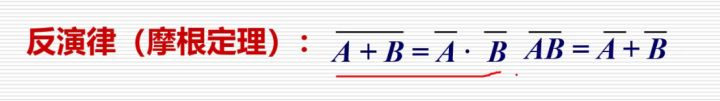
\includegraphics[width=0.7\textwidth, keepaspectratio]{2-3.png}
  \caption{交织器}
\end{figure}

接收到的数据逐行写入到去交织器中,再逐行写出码字用于信道译码

\begin{figure}[h]
  \centering
  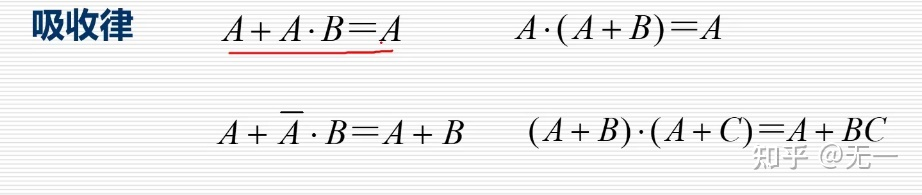
\includegraphics[width=0.7\textwidth, keepaspectratio]{2-4.png}
  \caption{去交织器}
\end{figure}

由上图可以看到,在交织器的作用下,如果出现了连续的突发噪声(灰色的部分),在去交织后,噪声平均分到了第3、4、5、6行,成功将较长的突发噪声转变成了随机噪声。

\section{经典信道编码发展}
在香农提出了信道编码定理后,出现了许许多多的好的编码方案。它们都是围绕着在有着较大码长的基础上,又能够让最大似然概率译码的复杂度可以接受的方式构造的。例如Hamming码 、BCH码 、Rs码等线性分组码以及卷积码。Hamming码由Hamming提出,但是它只能纠正一个错误,后来的BCH码则可以纠正多个错误。RS码于1960年构造出来,是BCH码的一个子类,由于其优异的纠错能力以及抗随即突发噪声能力,被广泛运用于CD、磁盘等存储领域。卷积码在1955年由Elias提出,后续Viterbi提出的 Viterbi译码算法被证明是卷积码的最大似然译码算法,1974 年Bahl、Cocke、Jelinek 和 Raviv(BCJR)提出了最大后验概率(MAP)译码算法,加快了卷积码的应用。
它们大多是使用代数实现编码,并以Hamming距离为度量。设计的目标是要最大化码字之间的Hamming距离从而获得优异的性能。这些编码方法都与香农极限有着较大的距离,在后续的发展中,又出现了级联码的方法,这种方法能够在不增加译码复杂度的情况下,增加码字长度,大大提高了编码的性能。但是要想达到香农极限,还是有比较大的一段距离。


\section{现代信道编码}
现代信道编码的发展始于1993年,那年的IEEE国际通信会议上,由Berrou, Glavieux, 和Thitimajshima首次公开了Turbo码,引发了轰动,计算机的模拟结果显示,如果使用大小为65535的随机交织器,进行18 次迭代,在Eb/No≥0.7dB时,码率为1/2的turbo 码在AWGN信道上的误码率≤10~5, 达到了近Shannon限的性能。\cite{berrou1993near}这无疑将信道编码往前提了一大步。而在Turbo码被提出之前,LDPC码就已经被Gallager提出,但是由于基于迭代算法的LDPC码的计算量太大,受当时计算能力和理论的限制,LDPC码被认为是不适用的编码方法。后来随着时代的发展,Mackay等人发现,在使用迭代译码算法时,LDPC码能够无线逼近香农极限,这被称为LDPC码的再发现,人们开始对LDPC码重视起来。虽然LDPC码和Turbo码都能够无限逼近香农极限,但是这都是在计算机的模拟中得出的结果,并没有被理论上证明。而在2008年,Arikan提出了Polar码,并给出了严格的数学证明,这是第一个被理论上证明的能够达到香农极限的编码算法。

\subsection{Turbo码}
Turbo码是一种并行级联卷积码,被广泛认为是信道编码领域的一个里程碑,它在信道编码性能方面取得了巨大的突破。Turbo码的出现使得信道编码能够接近香农极限,提供了可靠的通信性能。

Turbo码编码器由两个并联的递归系统卷积编码器(RSC)和一个交织器组成。编码器的输出端共分为三个部分。

第一部分$O_1$直接输出信息序列,没有经过任何编码操作。这部分保留了原始信息的部分,起到了基本的传输作用。

第二部分$O_2$通过RSC编码器1对信息序列进行编码,并通过一个删余器输出。RSC编码器1将输入的信息序列进行递归系统卷积编码,增加了冗余度,提供了一定的纠错能力。删余器根据特定的规则对编码后的码字进行删减和保留,以减小编码后的数据量。

第三部分$O_3$先将信息序列通过交织器进行处理,然后经过RSC编码器2进行进一步的编码。交织器的作用是将信息序列进行打乱,使得连续的码字在传输中变得非连续,增加了抗干扰的能力。RSC编码器2对交织后的序列进行递归系统卷积编码,增加了更多的冗余度和纠错能力。最后,编码后的数据经过删余器输出。

\begin{figure}[h]
  \centering
  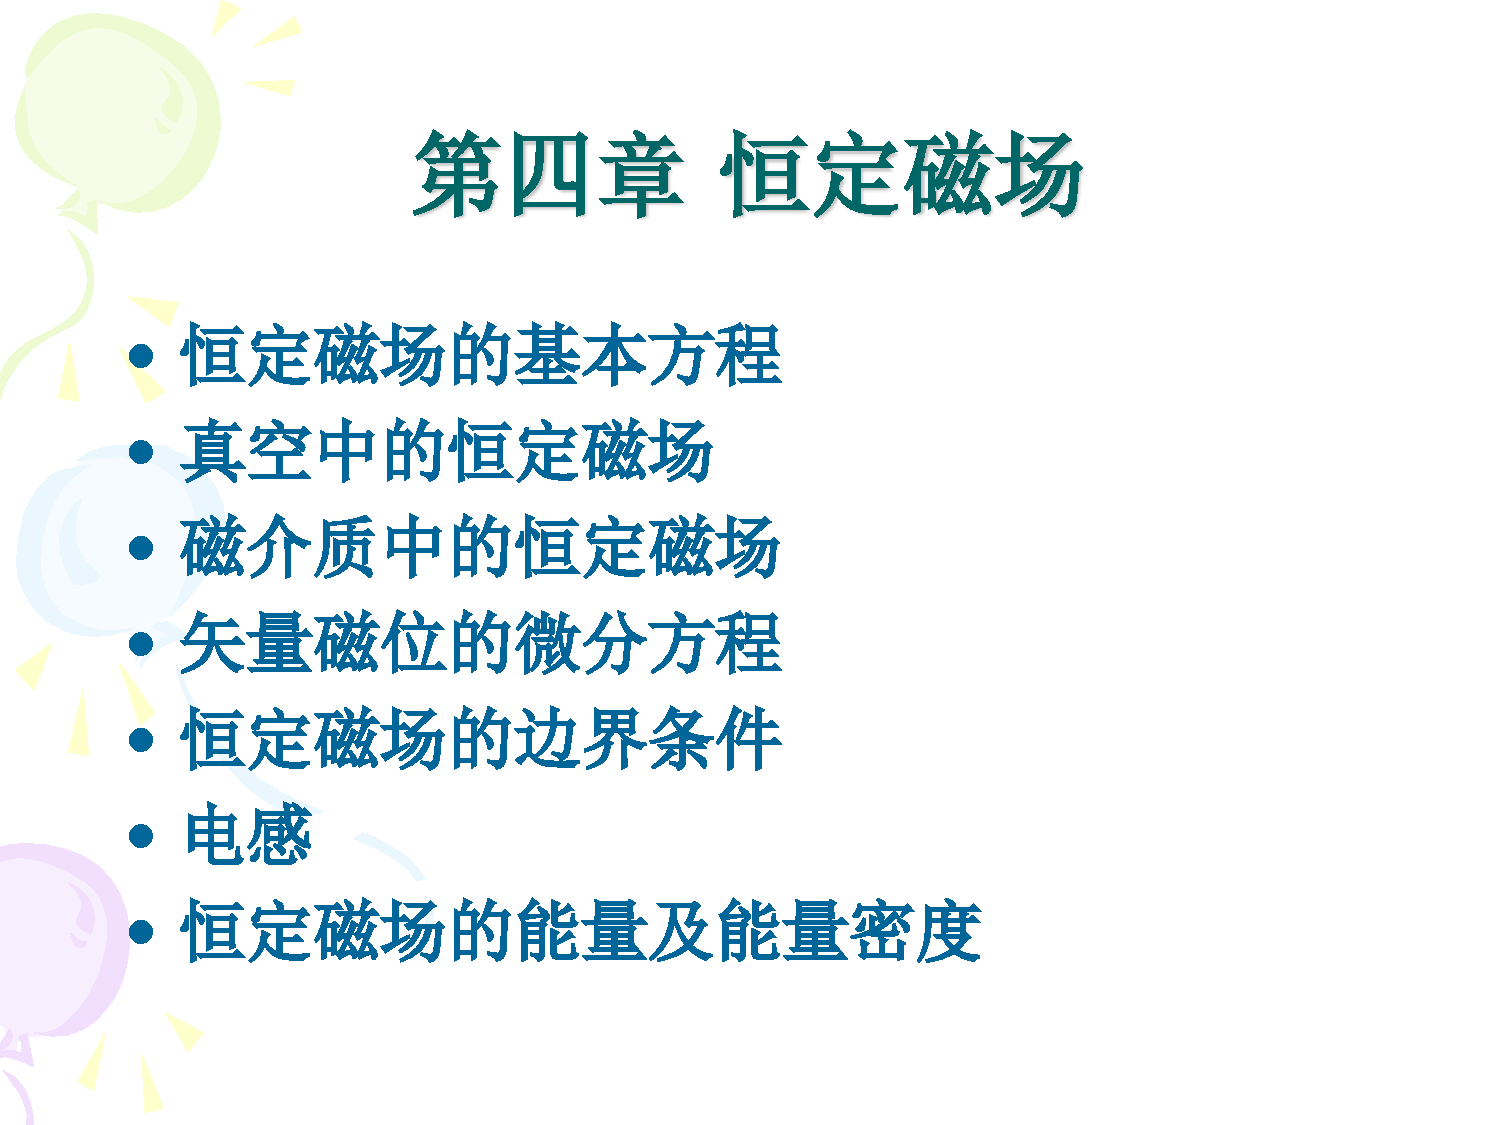
\includegraphics[width=0.4\textwidth, keepaspectratio]{4-1.png}
  \caption{Turbo码编码器}
\end{figure}

Turbo码的译码结构是Turbo码性能优异的重要原因,通过迭代译码,使得Turbo码的性能十分强大。Turbo码的解码过程与译码过程相互对应,可以看到译码器1有三个信号输入:$O_1$、$O_2$和$L_{e2}^*$,其输出$L_1$再与$O_1$和$L_{e2}^*$相减,得到外信息$L_{e1}$,$L_{e1}$经过交织器得到$L_{e1}^*$,并参与译码器2的译码。
译码器2也是三个输入:由$O_1$经过交织器后得到的$O_1^*$、$O_3$和$L_{e1}^*$,输出信号$L_2$与输入的$O_1^*$、和$L_{e1}^*$相减得到外信息$L_{e2}$,$L_{e2}$经过解交织得到$L_{e2}^*$,并参与译码器1的译码。其中,$L_2$经过解交织后得到的即为译码。

\begin{figure}[h]
  \centering
  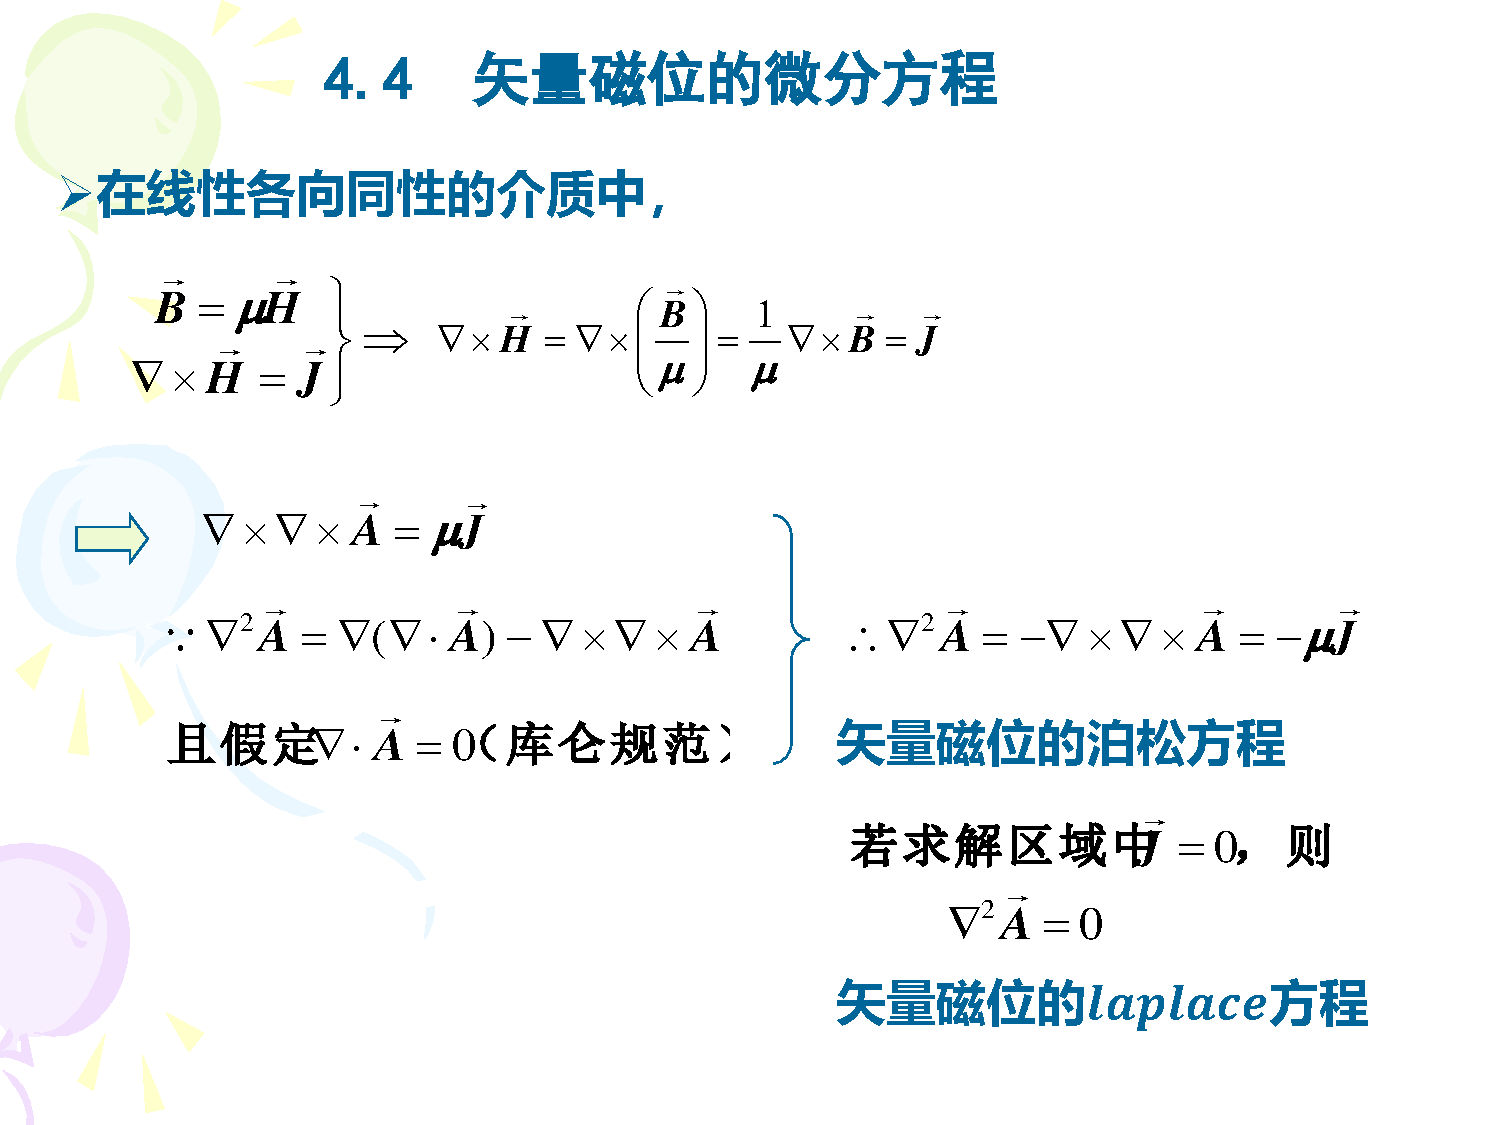
\includegraphics[width=0.8\textwidth, keepaspectratio]{4-2.png}
  \caption{Turbo码解码器}
\end{figure}
用公式表示$L_2$为
\begin{equation}
    L(b|r_1, r_2, \cdots, r_n) = L(r_1|b) + \sum_{i = 2}^{n} L(r_i|b) + L(b)
\end{equation}
\begin{equation}
    L(\hat{b}) = L_c(r) + L_e(\hat{b}) + L(b)
\end{equation}

由于Turbo码的译码过程通过不断迭代,接收信息的错误被不断地修正最后无限逼近香农限,整个过程如同汽车的涡轮机,由此得名Turbo。
得益于Turbo码的优异性能,它被广泛运用于3G技术和4G技术。然而Turbo码由于使用迭代译码算法,同时要进行交织和解交织,算法的复杂度大,延时也会加大。而且由于随机交织器的存在,使得Turbo码的理论分析比较困难,很多研究都是采用仿真分析的方法。同时,当信噪比比较大时,Turbo码的误码率下降速度开始放缓,存在地板效应。这些都是Turbo码发展需要解决的问题。

\subsection{LDPC码}
LDPC码又称低密度奇偶校验码。它是线性分组码的一种,也是奇偶校验码,因其校验矩阵是稀疏矩阵而得名。可将其与单奇偶校验码作对比。单奇偶校验码是在信息位后加一个监督码字使得整个码字的“1”的个数为奇数(或偶数)。其检验矩阵可以表示如下:
\begin{equation}
    H = \bigoplus_{i=1}^{n} a_i
\end{equation}
而对于长为n的LDPC码,其校验矩阵是一个m行,n列的稀疏矩阵。

相比于Turbo码,LDPC码有多个优点:1. 没有使用交织器,复杂度和时延都更小;2. 具有更好的误帧率性能,符合现代数字通信的要求;3. 错误平层低,逼近香农极限;4. 译码算法复杂度是线性的,译码器功耗更小,数据吞吐率更高。\cite{bai2016channel}

LDPC码的编码方法有很多。对长码、中长码、短码有不同的构造方法,可以分为两大类:1.随即构造和伪随机构造;2.结构化构造方法。其中结构化构造方法可分为代数构造方法和组合方法。不同的构造方法其优缺点也不同。在此,介绍一种由Richardson和Urbanke提出的将校验矩阵重新排列使得生成矩阵为下三角矩阵的编码方法,该方法的时间复杂度为$O(n^{1.5})$ \cite{richardson2001efficient}.
由于LDPC码也是线性分组码的一种,所以可以利用生成矩阵进行编码。由校验矩阵$H$进行变换,利用公式$GH^T = 0$得到生成矩阵G。再利用公式$C = UG$即可得到码字C。但是利用这个方法对H进行变换时会破坏校验矩阵的稀疏性,使得算法的复杂度变为$O(n^2)$,当码长n较大时,复杂度将会十分巨大。而减小复杂度的关键就在于尽可能地保证矩阵的稀疏性。Richardson方法就是将校验矩阵H进行行列变换,使得H矩阵右上角形成一个尽量大的下三角子矩阵。同时将码字C分成三部分$(s,p,q)$,其中s为信息位,p、q均为校验位,设三个部分的长度分别为x、y、z,如图所示;
$$
\begin{bmatrix}
     &  &  &  &  &  & & 1 & \cdots & \mathbf{0} \\
     &  & \mathbf{A} &  &  & \mathbf{B} & &  & \ddots &  \\
     &  &  &  &  &  & & \mathbf{T} &    & 1 \\
     &  &  &  &  &  & & &  &  \\
     &  & \mathbf{C} &  &  & \mathbf{D} & &  & \mathbf{E} &  \\
     &  &  &  &  &  &  & &    &  \\
\end{bmatrix}
$$
则运用公式(如下所示)就可以得到码字C。
\begin{equation}
    P_1^T = -\Phi^{-1}(-ET^{-1}A + C) 
\end{equation}
\begin{equation}
    P_2^T = -T^{-1}(As^T + BP_1^T)
\end{equation}
其中$\Phi = -ET^{-1}B + D$显然$|\Phi| \neq 0$.

除了用稀疏矩阵外,还可以使用Tanner图表示LDPC码。Tanner图是由节点和边组成的图形,其中,第一行的节点对应校验矩阵中的列,称为比特节点,第二行的节点对应校验矩阵中的行,称为校验节点,边则对应矩阵中的非零元素。例如,若校验矩阵为:
$$
H = \begin{bmatrix}
    1 & 0 & 1 & 1 \\
    0 & 1 & 1 & 1\\
\end{bmatrix}
$$
则Tanner图可以表示为如下所示:

\begin{figure}[h]
  \centering
  \includegraphics[width=0.3\textwidth, keepaspectratio]{4-3.png}
  \caption{校验矩阵H对应Tanner图}
\end{figure}


若一条路径的起始节点和终止节点重合,则构成环,环的长度是环中所含边的数目。短环会限制BP算法的译码性能,因此应注意不要出现短环,尤其是长度为4的环。
LDPC码的性能优异,是高速率大容量通信系统信道编码的首选方案。在5G标准上,LDPC码已经被确定为5G系统eMBB数据信道的编码方案。\cite{yu2018channel}


\subsection{Polar码}
相较于其他传统的编码方法,Polar码是最新提出的一种信道编码方法。由Arikan于2008年首次提出,它是目前唯一一种经过严格数学证明可以达到香农极限的编码方法。

Polar码又被称为极化码,其核心概念是信道极化理论。这种编码方法包括两个主要步骤:信道合并和信道分解。在信道合并过程中,当合并的信道数量趋近于无穷大时,一部分信道会变得非常可靠,接近无噪声信道的特性,而另一部分信道则会变得非常不可靠,接近全噪声信道的特性。这种现象被称为信道极化。

通过信道极化的过程,我们可以利用可靠的信道传输信息,而将不可靠的信道用于传输固定信息或者不传输任何信息。这种编码方法的优势在于,它利用了信道的特性,将可靠性分配给最适合传输信息的信道。如下图所示,展示了信道极化的过程。

\begin{figure}[h]
  \centering
  \includegraphics[width=0.75\textwidth, keepaspectratio]{4-4.png}
  \caption{Polar码信道极化过程}
\end{figure}

Polar码极化过程可以由以下过程为例。考虑BEC信道,信息被擦除的概率为p,则信道容量为1-p。现将两个BEC信道合并,如下图所示:

\begin{figure}[h]
  \centering
  \includegraphics[width=0.5\textwidth, keepaspectratio]{4-5.png}
  \caption{$W_2$信道}
\end{figure}

图中$W_2$表示BEC信道,由上图可知 $x_1 = u_1 \bigoplus u_2, x_2 = u_2$,矩阵表示为
\begin{equation}
    \begin{align*}
        [x_1, x_2] &= [u_1, u_2] \begin{bmatrix} 1 & 0 \\ 1 & 1 \end{bmatrix} \\
        &= [u_1, u_2]G_2
    \end{align*}
\end{equation}


可根据公式$u_1 = y_1 \bigoplus y_2$ 解码出$u_1$,此时,$u_1$传输成功的概率为$(1-p) \times (1-p)$;$u_2$可以直接由$y_2$得到,若$u_1$传输的是约定的信息,也可以根据公式$u_2 = u_1 \bigoplus y_1$得到,此时,$u_2$成功传输的概率为$1-p\times p$。显然$u_2$传输成功的概率比$u_1$高。再这两个信道合并的$W_2$信道与另一个$W_2$信道以同样的方式合并得到$W_4$、$W_8$...

\begin{figure}[h]
  \centering
  \includegraphics[width=0.6\textwidth, keepaspectratio]{4-6.png}
  \caption{$W_8$信道}
\end{figure}

随着合并信道不断增加,信道之间的擦除概率向着两个方向发展。在擦除概率$p=0.5$,合并信道为8个时,上图中$u_8$的擦除概率就已经下降到$0.0039$,$u_1$的擦除概率则达到了$0.9961$.而当合并信道足够多时,就会出现无噪信道和全噪信道,其中无噪信道所占比例为$1-p$,即香农极限。\cite{arikan2009channel}

由于极化码运用的是信道极化原理,因此在中短码长时,由于信道极化不充分,使用SC译码算法的效果不是很理想。为了进一步提高极化码在中长码时的性能,后续有很多优秀的译码算法被提出。例如,CRC辅助SCL算法。\cite{tal2015listdecoding}这是目前运用最广泛的Polar码的译码算法。其中CRC的作用有两个:一是改善高信噪比时的性能,二是筛选译码路径。

Polar的应用还不是很成熟,但作为第一个理论上证明了的能够达到香农极限的信道编码方法,它的发展未来可期。目前,Polar码被选作5G中eMBB应用场景的控制信道和编码方式,有着很强的潜力。


\section{结束语}
自从香农开创信息论并指出香农极限后,信道编码领域的理论和技术不断发展,目前已经形成了一个相当庞大的体系。从Hamming码到BCH码,再到Forney级联码等等,经典信道编码不断向香农限靠近,却始终有较大的差距。而Turbo码的出现实现了巨大跨越,将信道编码向香农极限前进了一大步,近乎达到香农极限。后续LDPC码的再发现,让人们离香农极限又进了一步。可惜的是,Turbo码和LDPC码由于复杂度的原因,未能形成比较完备的研究理论,只能通过计算机仿真的方式进行研究。Polar码的出现,让人们从理论上第一次达到了香农极限。虽然现在信道编码已经达到了它的最终目标——香农极限,但这并不意味着信道编码终结。编码方法的实际应用依旧是需要研究的方向。同时,现在的编码都是在码长充分的情况下达到香农极限,那么在码长受限的情况下,是否仍存在一个好的信道编码以达到香农极限,这样的问题还需要人们去探索。此外,香农研究的是点对点通信,对于现在愈发复杂的网络通信下的信道容量,还有很多是亟待人们去研究的。


\begin{thebibliography}{9}

\bibitem[1]{shannon1948}
Shannon, C. E. A Mathematical Theory of Communication[J]. Bell System Technical Journal, 1948, 27(3): 379--423.

\bibitem[2]{yu2018channel}
于清苹,史治平. 5G信道编码技术研究综述[J]. 无线电通信技术, 2018(1): 1--8.

\bibitem[3]{berrou1993near}
C. Berrou,A. Glavieux and P. Thitimajshima. "Near Shannon limit error-correcting coding and decoding:turbo-codes (1)", ICC'93, pp1064--1074. 1993

\bibitem[4]{bai2016channel}
白宝明 ,孙 成 ,陈佩瑶 ,等.信道编码技术新进 展[J].无 线电通信技术 ,2016,42(6):01-08


\bibitem[5]{richardson2001efficient}
Richardson T,Urbanke R.Efficient encoding of low-density parity-check codes[J].IEEE Trans.Info.Theory,2001-02,47(2):638-656


\bibitem[6]{arikan2009channel}Arikan E. Channel polarization: A method for constructing capacity-achieving codes for symmetric binary-input memoryless channels[J]. IEEE Transactions on information Theory, 2009, 55(7): 3051-3073.

\bibitem[7]{tal2015listdecoding}Tal Ⅰ, Vardy A. ListDecoding of Polar Codes[ J]. IEEE Transactions on Information Theory , 2015,61(5) :2213-2226

\end{thebibliography}

\end{document}
